\documentclass{article}
\usepackage[margin=1in]{geometry}
\usepackage{amsmath,amsthm,amssymb}
\usepackage{bbm,enumerate,mathtools}
\usepackage{tikz,pgfplots}
\usepackage{chessboard}
\usepackage[hidelinks]{hyperref}
\usepackage{multicol} % Problem 35

\newenvironment{question}{\begin{trivlist}\item[\textbf{Question.}]}{\end{trivlist}}
\newenvironment{note}{\begin{trivlist}\item[\textbf{Note.}]}{\end{trivlist}}
\newenvironment{references}{\begin{trivlist}\item[\textbf{References.}]}{\end{trivlist}}
\newenvironment{related}{\begin{trivlist}\item[\textbf{Related.}]\end{trivlist}\begin{enumerate}}{\end{enumerate}}


\begin{document}

\rating{2}{2}
Choose a point $p$ in $\mathbb{R}^2$, and consider all balls $\mathcal B_p(r)$
of radius $r$ centered at $p$. Let $f(\mathcal B_p(r))$ be the number of ``boxes'' of
$\mathbb{Z}^2$ that are partly contained in the interior of a ball.
\begin{figure}[ht!]
  \centering
  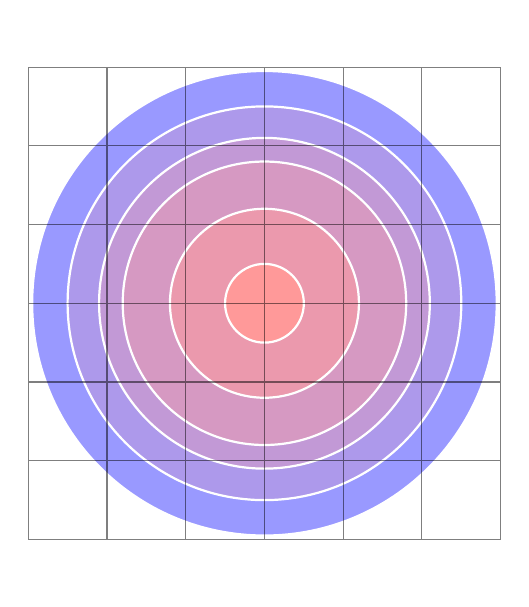
\begin{tikzpicture}
    \path (-3,-3.5) rectangle (3,3.5);
    \draw[white,thick,fill=red!0!blue!40] (0,0) circle (2.95);
    \draw[white,thick,fill=red!20!blue!40] (0,0) circle (2.5);
    \draw[white,thick,fill=red!40!blue!40] (0,0) circle (2.1);
    \draw[white,thick,fill=red!60!blue!40] (0,0) circle (1.8);
    \draw[white,thick,fill=red!80!blue!40] (0,0) circle (1.2);
    \draw[white,thick,fill=red!100!blue!40] (0,0) circle (0.5);
    \draw[opacity=0.5] (-3,-3) grid (3,3);
  \end{tikzpicture}
  ~
  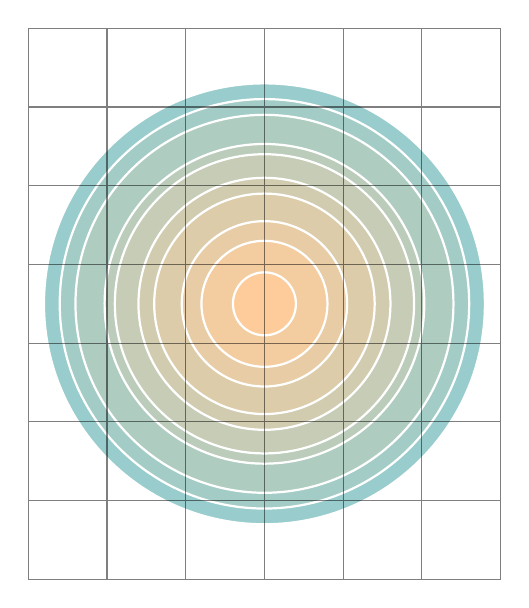
\begin{tikzpicture}
    \draw[white,thick,fill=orange!0!teal!40] (0,0.5) circle (2.8);
    \draw[white,thick,fill=orange!11!teal!40] (0,0.5) circle (2.6);
    \draw[white,thick,fill=orange!22!teal!40] (0,0.5) circle (2.4);
    \draw[white,thick,fill=orange!33!teal!40] (0,0.5) circle (2.03);
    \draw[white,thick,fill=orange!44!teal!40] (0,0.5) circle (1.9);
    \draw[white,thick,fill=orange!55!teal!40] (0,0.5) circle (1.6);
    \draw[white,thick,fill=orange!66!teal!40] (0,0.5) circle (1.4);
    \draw[white,thick,fill=orange!77!teal!40] (0,0.5) circle (1.05);
    \draw[white,thick,fill=orange!88!teal!40] (0,0.5) circle (0.8);
    \draw[white,thick,fill=orange!99!teal!40] (0,0.5) circle (0.4);
    \draw[opacity=0.5] (-3,-3) grid (3,4);
  \end{tikzpicture}
  \caption{
    When $p \in \mathbb{Z}^2$, the range of $f$ is $\{0,4,12,16,24,32,36,\dots\}$;
    when $p$ is in the middle of an edge, the range of $f$ is $\{0,2,6,8,12,16,20,22,26,34,38,..\}$;
    when $p$ has irrational coordinates, the range of $f$ is $\mathbb N$.
  }
\end{figure}

\begin{question}
  What are all possible sequences for varying $p$?
\end{question}

\begin{related}
  \item What if $f'$ counts the number of vertices in a circle?
    Or if $f''$ counts the number of boxes that are \textit{entirely} inside
    of a circle?
  \item What happens on other lattices, tilings, or higher dimensional analogs?
  \item How does this vary when the ``circles'' are generated by other metrics?
\end{related}

\begin{references}
  \item Problem 30.
  \item \url{https://codegolf.stackexchange.com/q/217444/53884}
\end{references}
\end{document}
